\chapter{Physical Properties of Capacitors and Inductors}
\label{chap:capInductorProperties}
So far we've looked at circuits with resistors, DC voltage supplies, and DC current supplies. We are about to dive into AC (time-varying) power sources, but before we do, we need to discuss two other passive elements besides resistors---the capacitor and the inductor. These circuit elements aren't very interesting in DC circuits, but they really shine when driven by AC sources. The capacitor and inductor set up internal electric and magnetic fields, respectively, when they are driven by a source that varies with time. Those fields store energy briefly rather than dissipating it away in the form of heat like resistors do. Capacitors and inductors are found in almost any electronic product you can buy today. Let's look at the physical properties of these two elements before we dig deeper and investigate their behavior in an AC circuit.
\section{Capacitor Geometry and Behavior}
\label{sec:capGeometryAndBehavior}
\begin{figure}[h!]
\centering
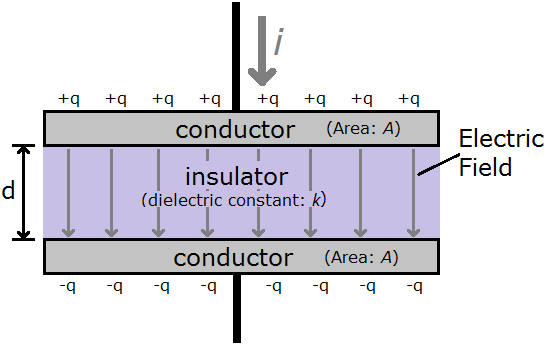
\includegraphics[width=10cm]{figures/capacitorAnnotated.png}
\caption{A capacitor is comprised of conductive plates separated by a dielectric (insulating) material. This allows an electric field to form between the plates, which is the mechanism by which a capacitor stores energy.}
\label{capInDetail}
\end{figure}
A capacitor is a circuit element that stores energy in the form of an electric field. The geometry of a capacitor is very simple; typically, a capacitor is comprised of two conductive plates separated by a layer of dielectric material. A diagram of such a device is shown in Figure \ref{capInDetail}. When a voltage source is applied across the device, electrons in the device are pulled toward the higher voltage plate of the capacitor. However, because there is not a conductive path between the plates, the higher-voltage plate builds up a net positive charge as its electrons are drawn to the positive terminal of the voltage source, and the lower voltage plate builds up a net negative charge as electrons pool there. The build-up of charge in a capacitor is related to the voltage across the capacitor according to the following expression:
$$
Q_c = C \cdot V_c
$$
When the voltage $V_c$ is built up across the plates, each plate has built up a charge of magnitude $Q_c$, but the higher voltage plate has charge of $+Q_c$, while the lower voltage plate has charge of $-Q_c$. This charge differential causes an electric field to form within the dielectric layer of the capacitor. The magnitude of this charge differential cannot grow indefinitely; eventually, the voltage of each of the plates of the capacitor will match those of the applied source, and current will cease to flow into and out of the device. 
\par
You can think of the \textbf{capacitance} for a device as a measure of how effective that device is at storing energy. The value for capacitance is based largely on the geometry of the device:
$$
C = \frac{k \cdot \epsilon_0 \cdot A}{d}
$$
In this definition, $k$ represents the \textit{dielectric constant} for the insulator material between the plates, $\epsilon_0$ is the \textit{electric permittivity of vacuum} ($8.85 \cdot 10^{-12}$F/m), $A$ is the area of each plate in the capacitor, and $d$ is the distance separating the plates. 
\par
Electric permittivity sounds really esoteric and complicated, but it's just a measure of how much charge must be built up across a medium to sustain a particular electric field. Ok, after having written that, I realize that electric permittivity \textit{is} a bit esoteric. Think about it this way: any molecule or atom can have its positively-charged nucleus and negatively-charged electron cloud pulled in opposite directions by an electric field. When that happens, the polarized atom or molecule works \textit{against} the electric field. Now, think about having a polarizable medium in between the plates of a capacitor. When voltage is applied across the capacitor and charge builds up on the capacitor plates, that forms an electric field between the plates. The medium between the plates is then polarized by the electric field, which works against the buildup of the field. Therefore, more charge is needed at the capacitor plates to create the electric field required by the applied voltage. 
\par
In contrast, vacuum has no particles to be polarized by an applied electric field. Because of that, the charge differential on the plates of the capacitor wouldn't have to fight any polarization of the vacuum in building up an electric field and such a capacitor would require \textit{less} charge across the plates to sustain a particular applied voltage. For this reason, vacuum has the lowest permittivity of any medium, and $\epsilon_0$ is used as a reference permittivity for other materials. In fact, the \textit{dielectric constant} ($k$) in the formula for capacitance above is a parameter that describes \textit{how many times larger} the permittivity of the dielectric layer material is than the permittivity of vacuum. When $\epsilon_0$ is multiplied by $k$, the result is the permittivity of the particular insulator material between the plates of the capacitor.
\par
The area and separation of the capacitor plates---$A$ and $d$, respectively---are purely spatial characteristics of the capacitor, as shown in Figure \ref{capInDetail}. We can increase capacitance by either decreasing the distance between the plates or increasing the area of the plates. In so doing, we would increase the total electric field strength in the dielectric, and thus increase the energy storage capacity for the device. We won't spend a lot of time analyzing the transient behavior of capacitors in this class, but the concepts of this section are good to keep in mind as we discuss the behavior of capacitors in circuits with AC (sinusoidally-varying) sources.
\par
Capacitance is measured in \textit{Farads} (F), which are very large units. In practice, it is most common to see capacitors within the range of picofarads ($10^{-12}$F) to hundreds of microfarads ($\sim100 \cdot 10^{-6}$F), and very uncommon to see capacitors of millifarad ($10^{-3}$F) capacitance or more.

\section{Inductor Geometry and Behavior}
\begin{figure}[h!]
\centering
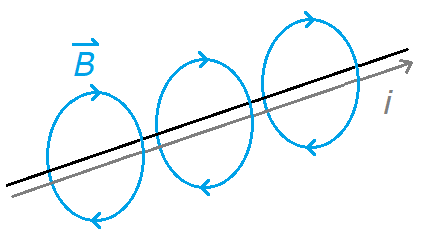
\includegraphics[width=10cm]{figures/magneticFieldInduction.png}
\caption{Current flowing through a wire ($i$) induces a magnetic field ($\vec{B}$) around that wire.}
\label{magneticFieldAroundWire}
\end{figure}

When current flows through a wire, a magnetic field is generated which curls around the wire as represented in Figure \ref{magneticFieldAroundWire}. If the wire is itself coiled, the magnetic field induced by the current flowing through the wire can reinforce itself, which is the principle by which inductors operate.
\begin{figure}[h!]
\centering
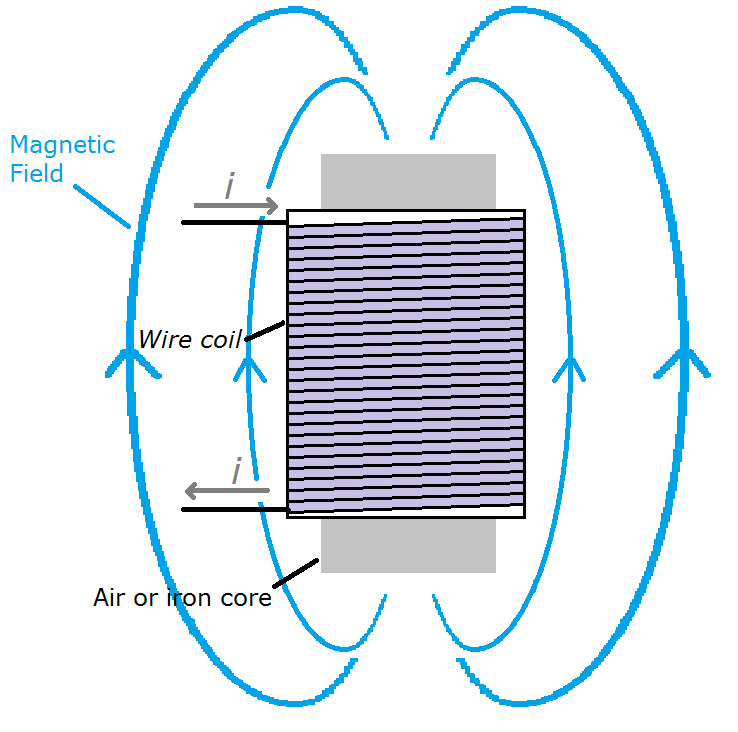
\includegraphics[width=10cm]{figures/inductorAnnotated.png}
\caption{An inductor is made of a coil of wire wrapped around a core made of air, iron, or other material. When current flows through the wire in the coil, it generates a magnetic field as indicated by the field lines in this diagram. The inductor stores energy in this field.}
\label{inductorInDetail}
\end{figure}
An inductor is simply a coil of wire wrapped around an air or iron core. When current flows through the inductor, it generates a magnetic field directed axially through the core. The \textit{magnetic flux} ($\Phi$) in the core of the inductor is defined as follows:
$$
\Phi = |\mathbf{B}| \cdot A
$$
In this definition, $|\mathbf{B}|$ is the magnitude of the magnetic field in the core, and $A$ is the cross-sectional area of the core. This flux is just part of what defines the \textbf{inductance}(L) of the device:
$$
L = N\cdot\frac{\mathnormal{d}\Phi}{\mathnormal{d}i_L}
$$
$N$ is the number of turns of wire in the inductor, $\Phi$ is the magnetic flux in the core, and $i_L$ is the current flowing through the inductor. Inductance is measured in Henries (H). In contrast to Farads, Henries are a practically-sized unit, and inductances on the order of single Henries are often encountered in practice.
\par
The physical behavior of inductors is not as easy to visualize as that of capacitors, but inductors store energy in their current-induced magnetic field. As the magnetic field in the coil of an inductor is building up or diminishing, a voltage difference across the inductor forms to counteract the change in the field. So, when there is no field inside the coil, energy is required to overcome the reactive voltage and build up the field. Conversely, once the field is present, any change in its amplitude causes another reactive voltage to form, which counteracts the change. This voltage puts energy back into the circuit from the field inside the inductor coil. If this is confusing, just remember that the field stores energy and it releases that energy back to the circuit in the form of voltage across the inductor. We will define the current-voltage relationships for the inductor and the capacitor later in this chapter.

\section{Steady-State Behavior of Capacitors and Inductors in Circuits}
In the previous section, we saw that the geometries of the capacitor and the inductor are really simple. Furthermore, if we didn't have electric or magnetic fields to consider, they would behave really simply, too. In this section, we are going to investigate the steady-state (DC) behavior of these devices in order to enhance our conceptual understanding of their behavior under eventually more dynamic conditions. 
\begin{figure}[h!]
\centering
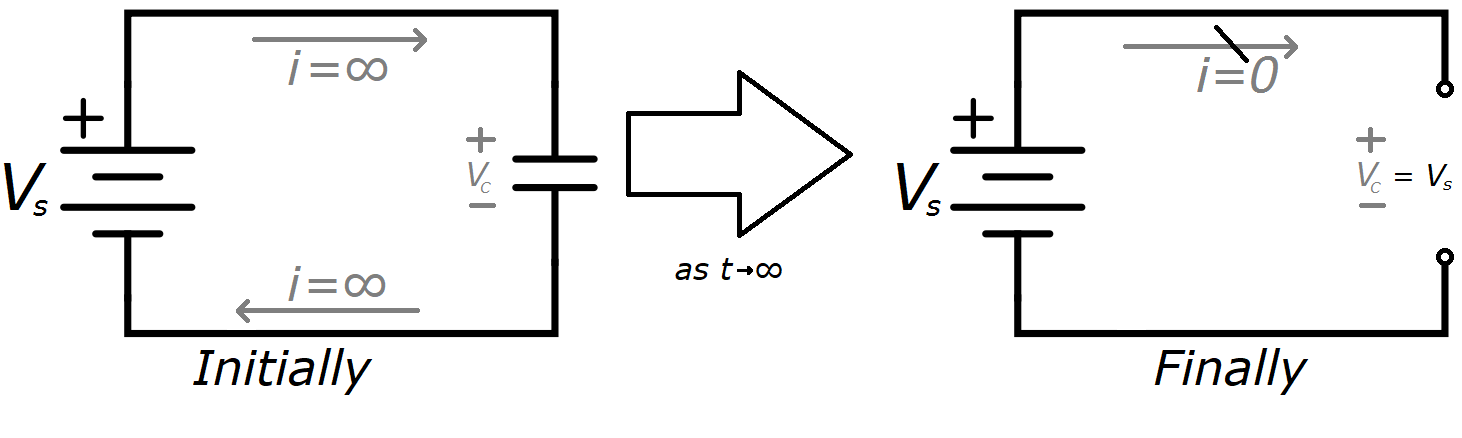
\includegraphics[width=13cm]{figures/capAndVoltage.png}
\caption{This circuit has just a voltage source and a capacitor---which is schematically represented as two unconnected parallel lines. At the moment when a voltage is applied across a capacitor, infinite current will flow into and out of the capacitor plates. This current will quickly decay as the capacitor voltage $C_V$ approaches the applied voltage $V_s$. Eventually, the capacitor acts as an open circuit with no current flowing in or out.}
\label{capSteadyState}
\end{figure}
\par
Let's consider the capacitor again for a moment. It has two disconnected conductive plates. By design, there is no path between them through which current can flow. However, when a voltage is applied across the capacitor, an initially very large current begins to flow which causes electrons to build up on the negative plate while other electrons are pulled off of the positive plate. This buildup of charge creates an electric field within the capacitor which resists further charge buildup. Because of this, the amplitude of the current flowing into and out of the capacitor decays rapidly as the voltage across the capacitor approaches the applied voltage value. Once the voltage across the capacitor reaches the value of the applied voltage, there is no more electron drift in the device, and it then acts as a simple open circuit. Figure \ref{capSteadyState} shows a diagram of this behavior. 
\begin{figure}[h!]
\centering
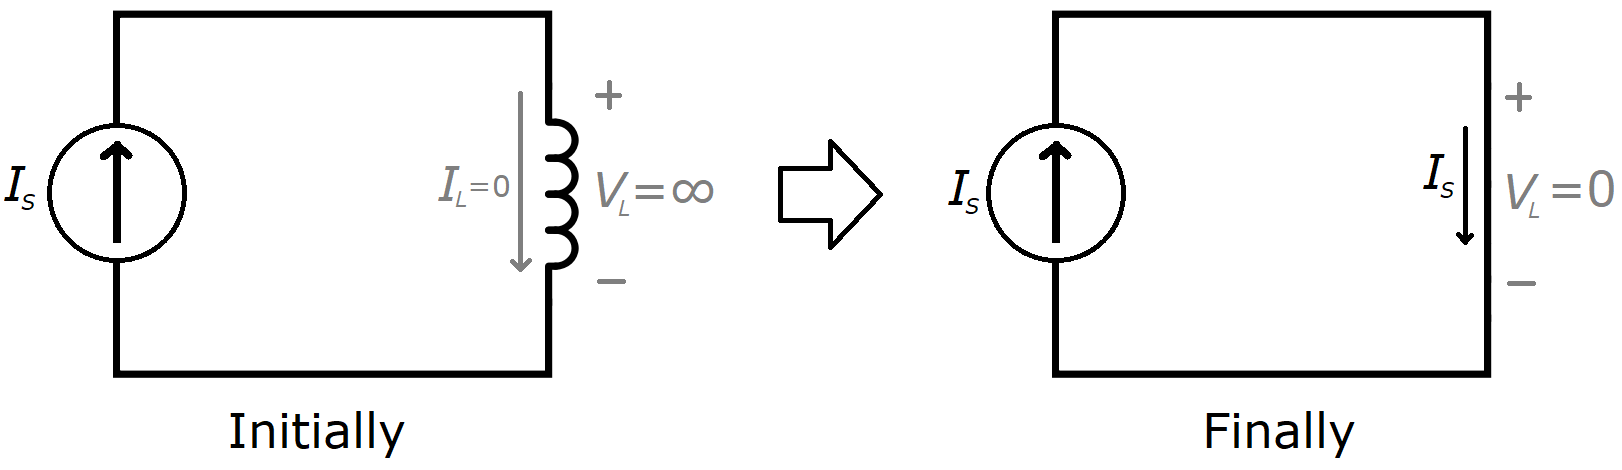
\includegraphics[width=13cm]{figures/inductorAndCurrent.png}
\caption{At the moment when a current is applied through an inductor, a very large reactive voltage forms across that inductor. However, as the inductor current approaches the applied current, the voltage across the inductor decays to zero, and then the inductor behaves like a wire.}
\label{inductorSteadyState}
\end{figure}
\par
The inductor, similarly, has very boring long-term steady-state behavior. As shown in Figure \ref{inductorSteadyState}, when a current is applied through the inductor, a very large voltage forms across the inductor in reaction to the current-induced magnetic field in the device. Initially, the current through the inductor is zero, but as it approaches the value of the applied current source, the magnitude of the magnetic field becomes stable and the voltage across the inductor diminishes to zero. Essentially, the inductor behaves just like a short circuit (i.e., a wire) once the magnetic field in the device stabilizes.
\begin{figure}[h!]
\centering
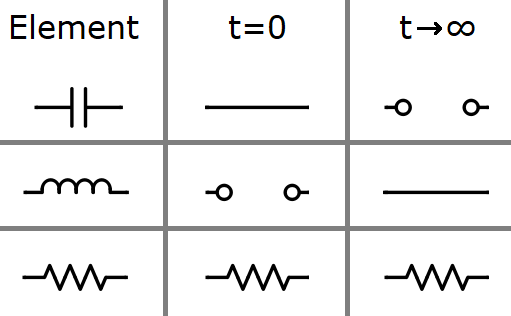
\includegraphics[width=10cm]{figures/RLClongTerm.png}
\caption{This table shows the behavior of all three passive circuit elements at the moment they are connected to a source, and after a long time has passed.}
\label{RLClongTerm}
\end{figure}
\par
To sum up the information of this section, the table in Figure \ref{RLClongTerm} concisely shows the initial and final behavior of all three passive circuit elements when they are connected to a DC power supply. The capacitor initially acts like a short circuit, but it behaves like an open circuit after some time. The inductor acts like an open circuit at first, but after some time it acts like a short circuit. And the resistor...just acts like a resistor at all times.

\section{Combining Inductors and Capacitors in Parallel and Series Configurations}
When multiple capacitors or multiple inductors are combined in one circuit, we can use some simple rules to determine an equivalent capacitance or inductance for the configuration. Let's start with inductors. If two or more inductors are in series, the equivalent inductance of the collection is the sum of all of the individual inductances. This makes sense given what we know about the geometry of an inductor; by putting multiple inductors in series with each other, we effectively increase the number of turns through which the magnetic flux passes. Also, if two or more inductors are connected in parallel, the total current flowing into them is split between the two inductors, which effectively reduces their equivalent inductance. Concisely:
$$
\textnormal{For }m\textnormal{ inductors in series:   }L_{eq} = \displaystyle\sum_{i=1}^mL_i
$$

$$
\textnormal{For }m\textnormal{ inductors in parallel:   }L_{eq} = \frac{1}{\displaystyle\sum_{i=1}^m\left(\frac{1}{L_i}\right)}
$$
\par
For capacitors, the rules are flipped; when multiple capacitors are combined in parallel, their equivalent capacitance is given by the sum of their individual capacitances. This makes sense if we think of adding a capacitor in parallel as adding surface area to the plates of a single capacitor. According to the equation for capacitance we saw in Section \ref{sec:capGeometryAndBehavior}, the capacitance increases with the area of the plates. If multiple capacitors are in series, however, the effective separation between their plates is equal to the sum of all the plate separations. This spreads the electric field out over a larger distance, and therefore the equivalent capacitance is less than the individual capacitances in the series. The rules for combining capacitances are:
$$
\textnormal{For }m\textnormal{ capacitors in parallel:   }C_{eq} = \displaystyle\sum_{i=1}^mC_i
$$
$$
\textnormal{For }m\textnormal{ capacitors in series:   }C_{eq} = \frac{1}{\displaystyle\sum_{i=1}^m\left(\frac{1}{C_i}\right)}
$$
\section{Derivation of the Voltage-Current Relationship for Capacitors and Inductors}
\textbf{Warning: calculus ahead.} The point of this section is to figure out how to relate current flowing through and voltage across both capacitors and inductors. If I use V = i $\times$Z (Ohm's Law) to do this, what is Z for capacitors and inductors? I answer that question in this section.
\par
To use the rules we learned about in Chapters \ref{chap:fundamentals} and \ref{chap:resistorRulesAndTricks} to analyze capacitor and inductor circuits, we need to be able to relate voltage across capacitors and inductors to current flowing through them. The mathematical expressions relating the physical relationships between current and voltage for both the capacitor and the inductor are, unfortunately, differential equations. For example, the current flowing into and out of a capacitor defines the change of voltage across that capacitor in the following way:
$$
i_C(t) = C \cdot \frac{d}{dt}V_C(t)
$$
Gross. However, we can define the capacitor and inductor impedances in a time-independent way as long as we assume the time-dependence of the driving source is sinusoidal with a single driving frequency. This may initially seem overly restrictive and possibly useless in practice, but as you will learn in your math classes if you haven't already, any time-varying signal can be represented as a linear superposition of sinusoids. Therefore, if we know how to characterize the impedance of a capacitor or inductor for a sinusoidal driving source with a single frequency, we could characterize the impedance of these elements for any range of frequencies.
\par
Let's manipulate the equation above until we are able to solve for $V_C/i_C$. This ratio is called the \textbf{impedance} of the capacitor, and it is represented by $Z_C$. (Ohm's Law is actually defined in terms of impedance as $V=i\times Z$, but we will discuss this more in the next chapter.)
\par
Let's first assume that 
$$
V_C(t) = V_0\cos(\omega t)
$$
and therefore 
$$
\frac{d}{dt}V_C(t)=-\omega V_0 \sin(\omega t)
$$
Combining these expressions yields the following:
$$
i_C(t) = C \cdot \left(-\omega V_0 \sin(\omega t)\right)
$$
Recall\footnote{As a student, I always used to love it when textbook authors would tell me to recall things I often hadn't ever heard before. If you find yourself in that position here, think about it for a minute, or just take my word for it and don't worry about recalling a thing!} that $-\sin(\omega t)$ differs from $\cos(\omega t)$ only by a phase shift of $\pi/2$:
$$
-sin(\omega t) = cos(\omega t + \pi/2)
$$
Now we want to separate the cosine term from the phase. To do this we will use, \textit{Euler's Formula}:
$$
e^{j\theta} = \cos{\theta} + j\sin{\theta}
$$
This formula introduces $j$, which is defined as $\sqrt{-1}$.\footnote{Before we go any further: in electrical engineering, we use ``$j$'' to denote $\sqrt{-1}$ instead of ``$i$''. We do this because ``$i$'' already denotes current, and for other historical reasons. Regardless of why, I will be using ``$j$'' in this way from now on.} We will explore imaginary numbers in more detail in the next chapter, but according to Euler's formula, multiplying $\cos(\omega t)$ by $e^{j\pi/2}$ is one way of introducing a phase shift of $\pi/2$. Therefore, we can rewrite our expression for $i_C$ in the following way:
$$
i_C(t) = e^{j\pi/2} C \omega \left(V_0 \cos(\omega t)\right)
$$
We now have our initial form of $V_C$ back in the equation, which means we're almost ready to solve for impedance. Before we do that though, we need to do something about that exponential term. Using Euler's formula again, we find that 
$$
e^{j\pi/2} = \cancelto{0}{\cos(\pi/2)} + j\cdot\cancelto{1}{\sin(\pi/2)}=j
$$
Finally, rewriting our expression for $i_C(t)$ yields 
$$
i_C(t) = j\omega C V_C(t)
$$
Therefore, for a sinusoidal driving source of frequency $\omega$, the impedance of a capacitor is
$$
Z_C = \frac{V_C}{i_C} = \frac{1}{j\omega C}
$$
This is better, but now we've traded time-dependence for ``imaginary-ness''. Which is worse? Well, time dependence is worse, obviously, but we will need to refresh our memories concerning imaginary numbers before we can do much with this impedance.
\par
The relationship between current and voltage for an inductor is complimentary to that for a capacitor:
$$
V_L(t) = L \cdot \frac{d}{dt}i_L(t)
$$
Assuming $i_L=I_0\cos(\omega t)$, and skipping most of the steps to get here, we find that 
$$
V_L = j\omega L i_L(t)
$$
Therefore, for a sinusoidal driving source of frequency $\omega$, the impedance of an inductor is
$$
Z_L = j\omega L
$$
\par
After the next chapter reintroduces complex algebra to you, firehose style, we will use the impedances derived above extensively to analyze circuits using resistors, capacitors, and inductors.
\section{Recap: Capacitors and Inductors}
You have now seen everything you need to know (and more) about capacitors and inductors for the purposes of this course. In the following chapters, we will apply the concept of impedance to analyze some circuits and to do some simple circuit design. For now, here are the highlights of this chapter listed succinctly:
\begin{description}
\item[Capacitance:] This is a measure of the energy storage capacity that a capacitor has. $$C = \frac{k \cdot \epsilon_0 \cdot A}{d}$$ where k is the relative permittivity of the dielectric material in the capacitor, A is the area of the capacitor plates, and d is the distance between the plates.
\item[Inductance:] This is a measure of the energy storage capacity an inductor has. $$
L = N\cdot\frac{\mathnormal{d}\Phi}{\mathnormal{d}i_L}
$$ where N is the number of wire turns for the inductor, $\Phi$ is the flux of the magnetic field through the inductor, and $i_L$ is the current flowing through the inductor that creates the magnetic field.
\item[Equivalent Inductance:] The rules for combining inductors are similar to the rules for combining resistors. 
$$
\textnormal{For }m\textnormal{ inductors in series:   }L_{eq} = \displaystyle\sum_{i=1}^mL_i
$$

$$
\textnormal{For }m\textnormal{ inductors in parallel:   }L_{eq} = \frac{1}{\displaystyle\sum_{i=1}^m\left(\frac{1}{L_i}\right)}
$$

\item[Equivalent Capacitance:] The rules for combining capacitors are the opposite of the rules for combining resistors.
$$
\textnormal{For }m\textnormal{ capacitors in parallel:   }C_{eq} = \displaystyle\sum_{i=1}^mC_i
$$

$$
\textnormal{For }m\textnormal{ capacitors in series:   }C_{eq} = \frac{1}{\displaystyle\sum_{i=1}^m\left(\frac{1}{C_i}\right)}
$$

\item[Capacitor Impedance:] $Z_C = \frac{1}{j\omega C}$
\item[Inductor Impedance:] $Z_L = j\omega L$
\end{description}
